% @Author: Athul Vijayan
% @Date:   2014-05-09 13:56:20
% @Last Modified by:   Athul
% @Last Modified time: 2015-09-02 00:21:06

\documentclass[11pt]{article}
\usepackage[utf8]{inputenc}
\usepackage[a4paper, margin=1in]{geometry}
\usepackage{amsmath}
\usepackage{amssymb}
\usepackage{graphicx}
\usepackage[toc,page]{appendix}
\usepackage{color}
\usepackage{subcaption}
\usepackage{placeins}
\usepackage{rotating}
\usepackage{wrapfig}
\usepackage{bm}
\usepackage[normalem]{ulem}
\usepackage[table]{xcolor}
\newcommand{\HRule}{\rule{\linewidth}{0.2mm}} % Defines a new command for the horizontal lines, change thickness here
\usepackage{hyperref}
\hypersetup{
    colorlinks,
    citecolor=black,
    filecolor=black,
    linkcolor=black,
    urlcolor=cyan
}
\usepackage{array}
\renewcommand{\P}{\mathbb{P}}
\newcolumntype{L}[1]{>{\raggedright\let\newline\\\arraybackslash\hspace{0pt}}m{#1}}
\newcolumntype{C}[1]{>{\centering\let\newline\\\arraybackslash\hspace{0pt}}m{#1}}
\newcolumntype{R}[1]{>{\raggedleft\let\newline\\\arraybackslash\hspace{0pt}}m{#1}}
\newcommand{\rulesep}{\unskip\ \vrule\ }

%----------------------------------------------------------------------------------------
%   TITLE PAGE
%----------------------------------------------------------------------------------------

\newcommand*{\titleGM}{\begingroup % Create the command for including the title page in the document
\hbox{ % Horizontal box
\hspace*{0.2\textwidth} % Whitespace to the left of the title page
\rule{1pt}{\textheight} % Vertical line
\hspace*{0.05\textwidth} % Whitespace between the vertical line and title page text
\parbox[b]{0.75\textwidth}{ % Paragraph box which restricts text to less than the width of the page

{\noindent\Huge\bfseries  Neural data analysis}\\[2\baselineskip] % Title
{\large \textit{Notes}}\\[4\baselineskip] % Tagline or further description
{\Large \textsc{Athul Vijayan}} % Author name

\vspace{0.5\textheight} % Whitespace between the title block and the publisher
}}
\endgroup}


\begin{document}
% \titleGM % This command includes the title page
\tableofcontents

% =========================== content =========================
\newpage
\section{Introduction} % (fold)
\label{sec:introduction}
\subsection{Background} % (fold)
\label{sub:background}

% subsection background (end)
\subsection{Experiment} % (fold)
\label{sub:experiment}
Virus expressing GCaMP6f was injected into the V1 of mice. Approximately 3 weeks post infection, mice were imaged under a 2-photon microscope while sinusoidal drifting gratings were presented on a computer screen placed 3 inches from the mouse (1 degree of visual space $\sim$ 21.3 pixels on the screen). The stimulus was varied as:
\begin{enumerate}
    \item Sinusoidal drifting gratings at 16 different directions (0:22.5:337.5). Spatial frequency was fixed at 0.03 cycles per degree.
    \item Each direction was repeated 10 times (i.e. 10 trials per direction). Directions are presented in a randomized order.
    \item Each direction was presented for 2s and was always preceded by a 4s gray screen. Therefore the total duration of the stimulus is 6s.
    \item Calcium signals (GCaMP6f in awake mice) were acquired from awake mice at 20 frames per seconds. Thus, sampling rate is 20Hz.
\end{enumerate}
 
% subsection experiment (end)

\subsection{Aim} % (fold)
\label{sub:aim}
\begin{itemize}
    \item To map orientation tuning responses of excitatory pyramidal neurons in V1.
    \item To determine response reliability at preferred orientation.
    \item To determine signal and noise correlations between neuron as a function of orientation tuning.
\end{itemize}
% subsection aim (end)

\section{Dataset} % (fold)
\label{sec:dataset}

\textbf{Notes about Data.mat}\\
Data.mat contains 4 entries:
\begin{enumerate}
    \item Data.rawF =  raw fluorescence values. Matrix size = number of cells x number of frames.
    \item Data.dFF    = fluorescence normalized to baseline (dFF =  (F-F0)/F0, where F0 is the baseline fluorescence computed using a sliding window of 400 frames). Same size as above.
    \item Data.Spks  = inferred spike rate using the Vogelstein deconvolution algorithm. Same size as above.
    \item Data.StimSeq = contains sequence of directions presented during that experiment. Vector size = 160 x 1.
\end{enumerate}
\textbf{Notes about Ori.mat}\\
Ori.mat contains 20 entries. The most pertinent entries are:
\begin{enumerate}
    \item Ori.OSI = orientation selectivity indices of the neurons
    \item Ori.OrFit = double-wrapped Gaussian fits
    \item Ori.OrFitQuality  = goodness of Gaussian fits. (Higher the percentage value, the better the fit)
    \item Ori.Width = tuning width in degrees
    \item Ori.PrefOri = preferred orientation
    \item Ori.SpkResponse = Contains neural responses for each cells sorted according to the different directions. Size: 1xNumber of cell Cell array. Each cell entry contains a 1x Number of Direction Cell array, which contains a Number of Frames x Trials matrix.
\end{enumerate}

\subsection{Restructuring the data} % (fold)
\label{sub:restructuring_the_data}
There are 19200 Ca readings for each mouse. The experiment is done using 16 different stimuli, Let us think of it as 16 classes. The angle of the drifting pattern changes between the classes. It is implicit that $0^{o}$ and $180^{o}$ will have same orientation, but the direction of drifting will be opposite.\\
First, the data is split into 16 parts corresponding to each class. There are 10 trials for each class. The data is split into 160 subsequences of $19200/160 = 120$ length. Now this is a time-series of 120 points for each trial, and there are ten sets of data for each class.\\
120 points in the data represents 6 seconds of brain activity. Out of the 6 seconds, first 4 seconds (80 samples for sampling frequency of 20Hz) correspond to no-stimuli (or Gray stimuli). This represents the background activity of the neuron. The last 40 samples show the response for the intended stimuli.
\begin{itemize}
    \item cellData{i} contains all data for neuron i
    \item cellData{i} is a 160$\times$121 matrix.
    \item Each row represents a single experiment. and corresponding gray duration.
    \item In a row first 120 entries show the time series data of 6 seconds (120 samples) long trial. First 4s (80 samples) gray time and last 2s (40 samples) stimuli time.
    \item Last column contain the angle of visual stimuli in radians. (class)
\end{itemize}

% subsection restructuring_the_data (end)

\section{Analysis} % (fold)
\label{sec:analysis}
Analysis is broken down into various problem statements. Various methods are considered for each of the problem statements.
\subsection{Quantifying the neuron activity} % (fold)
\label{sub:quantifying_the_neuron_activity}
The 120 point time series provide the activity of single cell in response to a particular stimulus in a trial. The activity of cell has to be studied. The first 80 samples are expected to have spikes due to only background activity, as the stimulus was gray during that time. Peaks in Ca concentration denotes the spikes in the neuron. From neuroanatomy, spike rate is a good quantify to measure neuron activity. In Calcium imaging, the amplitudes corresponds to Ca ion concentration. From the neuron models, more the Ca concentration, more is the spike rate. Following methods are used for quantifying spike rate.\\
Using various methods, a time sequence $F_t$ is calculated. $F_t$ represents the spiking activity of neuron. A relatively large $F_t$ represents a spike and small corresponds to no-spike. Number of spikes in an interval is what we seek. In the 120 sample data, $F_t$ of size 120 is found using various methods. Finally, spike rate is calculated by subtracting the background activity from the response.
$$spikeRate = \frac{\sum_{n=81}^{120} F_n}{40} - \frac{\sum_{n=1}^{80} F_n}{80}$$
Various methods for finding $F_t$ is the first problem statement. Following approaches are made to solve this.
\subsubsection{Thresholding } % (fold)
\label{ssub:thresholding}


% subsubsection thresholding (end)

\subsubsection{Moving Average model} % (fold)
\label{ssub:moving_average_model}

% subsubsection moving_average_model (end)

% subsection quantifying_the_neuron_activity (end)

\subsection{Estimating orientation selectivity of neuron} % (fold)
\label{sub:estimating_orientation_selectivity_of_neuron}
\subsubsection{Selectivity Index measures - OSI, DSI} % (fold)
\label{ssub:traditional_selectivity_measures_oi_di_and_osi}
OI and DI are used as the normalized measures of ``peak to trough'' orientation selectivity and direction selectivity.
These quantities are defined as:
\begin{align}
    OSI &= \frac{(R_{pref\_ori} - R_{orth})}{(R_{pref\_ori} + R_{orth})}\\
    DSI &= \frac{(R_{pref} - R_{null})}{(R_{pref} + R_{null})}
\end{align}
The response at the preferred orientation $R_{pref\_ori}$ and the response at the preferred direction $R_{pref}$ can be determined in different ways. In some measures, these are taken to be the best response to one of the stimulus orientations or directions that was explicitly measured; that is, if we measure responses at stimulus directions $\theta_1, \cdots, \theta_n$, then we choose the response at the best $\theta_i$ . In other measures, we perform a fit to the tuning curve, and choose the maximum value of the fit as $R_{pref\_ori}$ or $R_{pref}$ .
% subsubsection traditional_selectivity_measures_oi_di_and_osi (end)

\subsubsection{Circular variance of direction and orientation} % (fold)
\label{ssub:circular_variance_of_direction_and_orientation}
As discussed in the paper, Circular variance is a more robust quantifier of orientation and direction selectivity. A scalar value representing the neuron response is extracted from the 6s long time series for each of the orientations and directions (There are 8 orientations and 16 directions). As we have 10 trials for each class, we will have 160 such values for each neuron.\\
The values are first expressed as vectors in the orientation space. The vector sum of the values provide the `preferred orientation'; Magnitude should indicate how much orientation selective the neuron is.\\
Let $R(\theta)$ be the response of neuron to angle $\theta$ and we denote the `preferred direction' as $\theta_{pref}$.
Normalized vector sum in orientation and direction space is found as.
\begin{align}
    L_{ori} &= \frac{\sum_{k} R(\theta_k) exp(2\theta_k)}{\sum_{k} R(\theta_k)}\\
    L_{dir} &= \frac{\sum_{k} R(\theta_k) exp(\theta_k)}{\sum_{k} R(\theta_k)}
\end{align}
\begin{itemize}
    \item Neurons with orientation selectivity are expected to have high $L_{ori}$.
    \item Simple cells are orientation selective, but less direction selective. They are expected to have large $L_{ori}$ and small $L_{dir}$.
    \item Complex cells are orientation selective as well as direction selective. They are expected to have both large $L_{ori}$ and large $L_{dir}$.
\end{itemize}
Circular orientation variance and direction variance is given as
\begin{align}
    CirVar = 1 - |L_{ori}|\\
    DirCirVar = 1- |L_{dir}|
\end{align}
Following shows plots of orientation and direction selectivity of various kinds of neurons.
\begin{enumerate}
    \item \textbf{Orientation selective simple cell}\\
    Refer Figure~\ref{max_cirvar}
    \begin{figure}
    \centering
    \caption{Orientation selective simple cell}
    \label{max_cirvar}
    \begin{subfigure}{.48\textwidth}
        \centering
        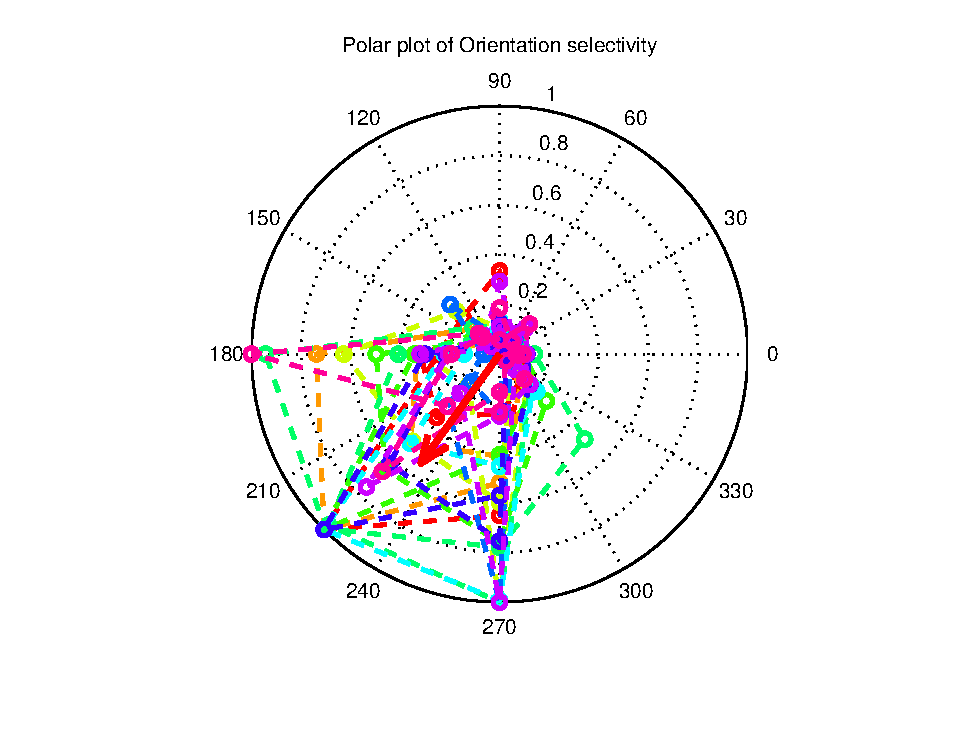
\includegraphics[width=\linewidth]{plots/max_cirvar_ori}
        \caption{Orientation selectivity plot of an orientation selective simple cell. Each curve shows a trial. Note that the cell is sensitive to an optimal orientation. The red arrow represents the direction and magnitude of orientation selectivity}
    \end{subfigure}
    \rulesep
    \begin{subfigure}{.48\textwidth}
        \centering
        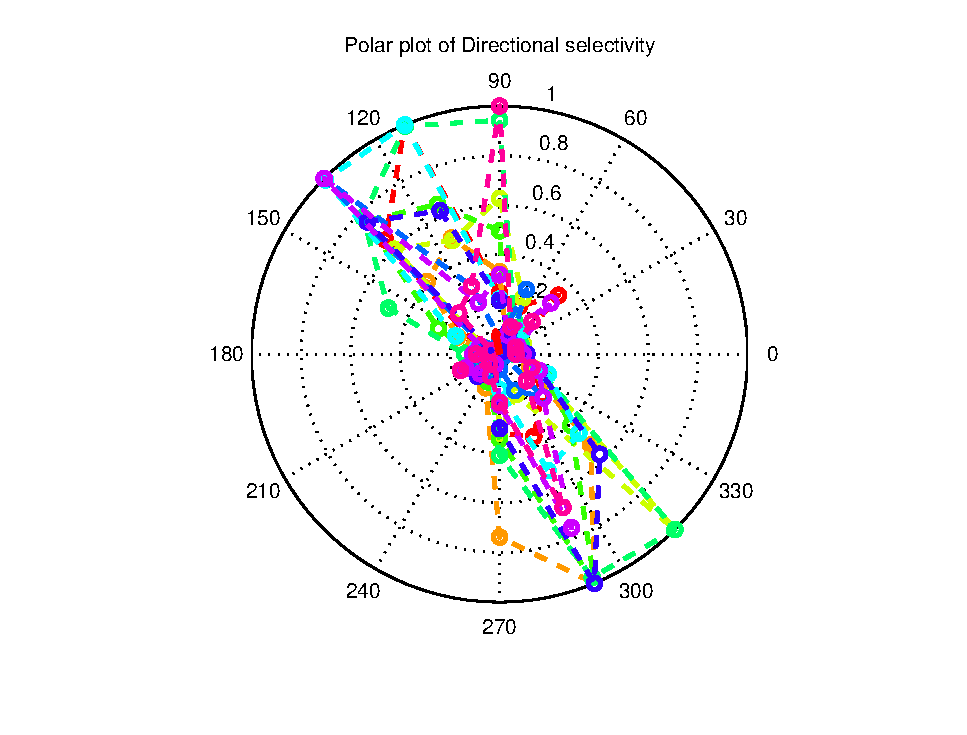
\includegraphics[width=\linewidth]{plots/max_cirvar_dir}
        \caption{Directional selectivity plot of an orientation selective simple cell. Each curve shows a trial. Note that the cell is not selective to direction, but is sensitive to orientation. The red arrow represents the direction and magnitude of direction selectivity}
    \end{subfigure}
    \end{figure}
    \item \textbf{Direction selective complex cell}\\
    Refer Figure~\ref{max_dircirvar}
    \begin{figure}
        \centering
        \caption{Direction selective complex cell}
        \label{max_dircirvar}
        \begin{subfigure}{.48\textwidth}
            \centering
            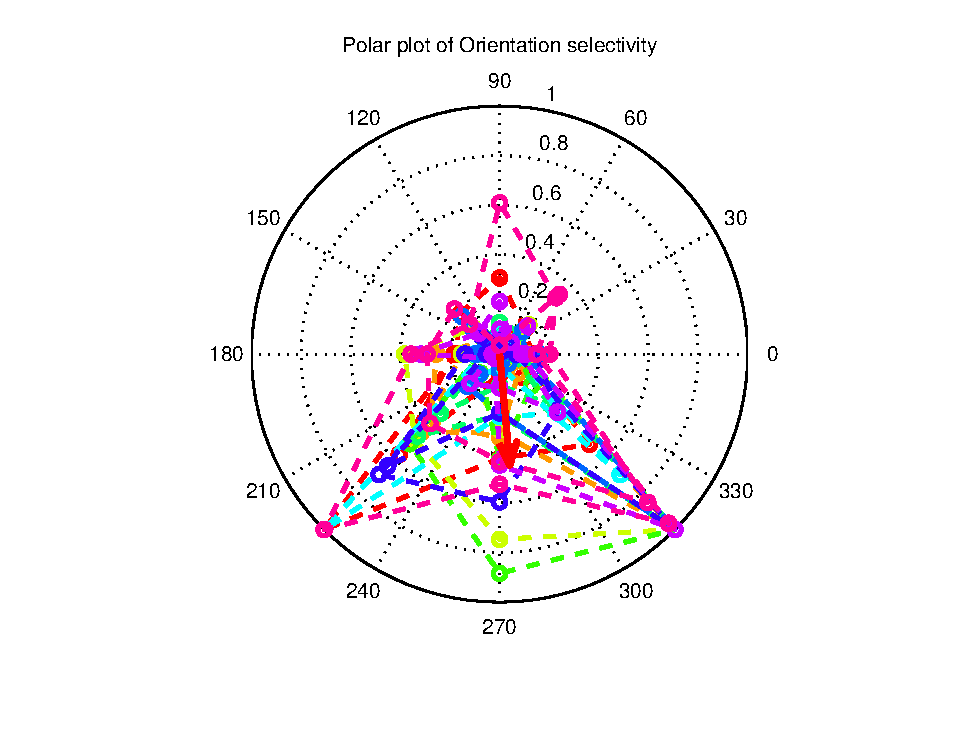
\includegraphics[width=\linewidth]{plots/max_dircirvar_ori}
            \caption{Orientation selectivity plot of an direction selective complex cell. Each curve shows a trial. Note that the cell is sensitive to an optimal orientation. The red arrow represents the direction and magnitude of orientation selectivity}
        \end{subfigure}
        \rulesep
        \begin{subfigure}{.48\textwidth}
            \centering
            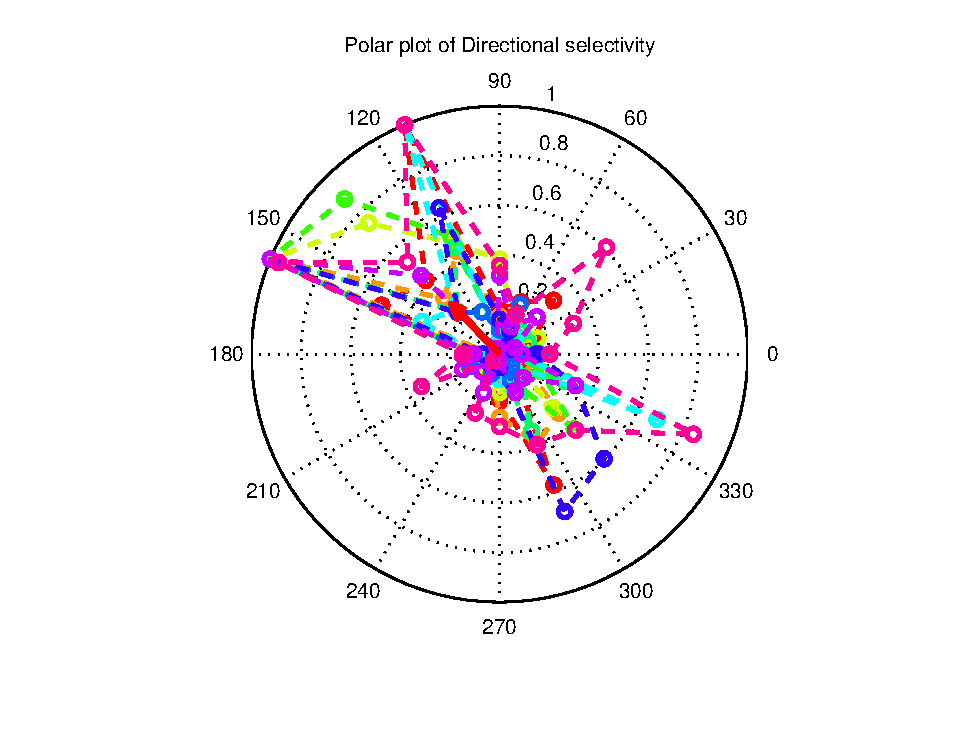
\includegraphics[width=\linewidth]{plots/max_dircirvar_dir}
            \caption{Directional selectivity plot of an direction selective complex cell. Each curve shows a trial. Note that the cell is selective to direction as well as orientation. The red arrow represents the direction and magnitude of direction selectivity}
        \end{subfigure}        
    \end{figure}
    \item \textbf{Orientation and direction Un-selective cells}\\
    Refer Figure~\ref{min_cirvar}
    \begin{figure}
        \centering
        \caption{Orientation and direction Un-selective cells}
        \label{min_cirvar}
        \begin{subfigure}{.48\textwidth}
            \centering
        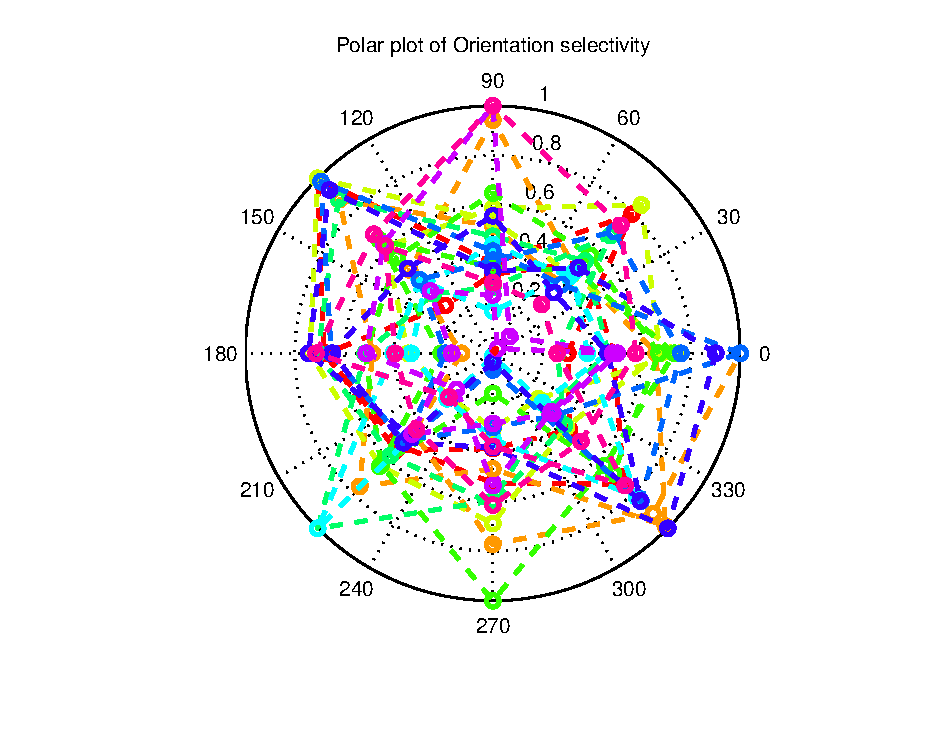
\includegraphics[width=\linewidth]{plots/min_cirvar_ori}
            \caption{Orientation selectivity plot of an Orientation and direction Un-selective cell. Each curve shows a trial. Note that the cell is uniformly sensitive to all orientations. The red arrow represents the direction and magnitude of orientation selectivity. Note the small magnitude}
        \end{subfigure}
        \rulesep
        \begin{subfigure}{.48\textwidth}
            \centering
            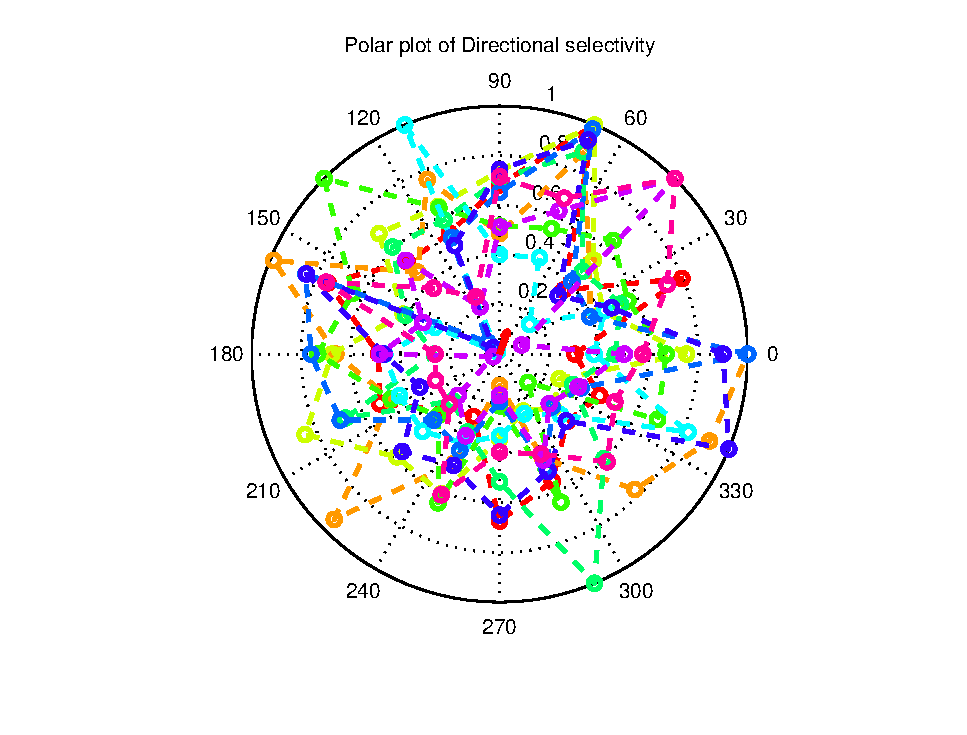
\includegraphics[width=\linewidth]{plots/min_cirvar_dir}
            \caption{Directional selectivity plot of an Orientation and direction Un-selective cell. Each curve shows a trial. Note that the cell is uniformly sensitive to all directions. The red arrow represents the direction and magnitude of direction selectivity. Note the small magnitude}
        \end{subfigure}
    \end{figure}
\end{enumerate}

% ======================= References ==========================
\newpage
\bibliographystyle{plain}
% argument is your BibTeX string definitions and bibliography database(s)
% \bibliography{test}
\bibliography{../../bibliography/imgProc}
\end{document}